\documentclass[11pt]{article}

\usepackage{graphicx}
\usepackage{url}
\usepackage{hyperref}

\begin{document}

\begin{center}
{\Large \bf Building the VMW Raspberry Pi / AY-3-8910 Chiptune Player}\\
\url{http://deater.net/weave/vmwprod/hardware/ay-3-8910/}\\
by Vincent M. Weaver\\
2 June 2017
\end{center}

\begin{center}
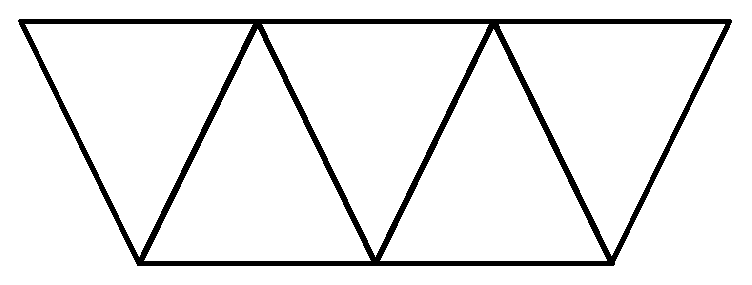
\includegraphics[width=1in]{figs/vmw}\\
A VMW Hardware Production
\end{center}

\section{Introduction}

This is a work in progress.  I will update it as I complete more
of the project.

%%%%%%%%%%%%%%%%%%
%%%%%%%%%%%%%%%%%%
\section{Building}
%%%%%%%%%%%%%%%%%%
%%%%%%%%%%%%%%%%%%

%%%%%%%%%%%%%%%%%%%%%%%%%%%%%%%%%%%%%%%%%%%%
\subsection{The Primary Sound Board ``hat''}
%%%%%%%%%%%%%%%%%%%%%%%%%%%%%%%%%%%%%%%%%%%%

\begin{table}
\caption{Sound Board Parts.~\label{table:sound_parts}}
\centering
\begin{tabular}{|c|c|c|c|r|r|}
\hline
NAME		& WHERE		& PART\#                  & QTY	& PRICE	   & TOTAL \\
\hline
\hline
PCB		& OSH Park	& VMW-CHIPTUNE-SOUND-MK1  & 1	& \$45.08  & \$45.08 \\
\hline
PCB		& OSH Park	& VMW-CHIPTUNE-SLIDER-MK1 & 1   &  \$2.80  &  \$2.80 \\
\hline
AY-3-8910	& eBay		& AY-3-8910		  & 2	&  \$3.00  &  \$6.00 \\
\hline
40-pin sockets	& Jameco	& 112311		  & 2	&  \$0.49  &  \$0.98 \\
		&		& 40-pin 0.60" wide       &     &	   &         \\
\hline
16 pin socket	& Jameco	& 37402                   & 2	&  \$0.75  &  \$1.50 \\
		&		& 16-pin 0.3"		  &     &          &         \\
\hline
14-pin osc sock	& Jameco	& 133006	          & 1	&  \$0.65  &  \$0.65 \\
		&		& 4-pin oscillator socket &     &	   &	     \\
\hline
14-pin socket	& Jameco	& 37197			  & 3	&  \$0.65  &  \$1.95 \\
		&		& 14-pin 0.3"		  &     &          &         \\
\hline
8 pin socket	& Jameco	& 51626                   & 1	&  \$0.45  &  \$0.45 \\
		&		& 8-pin 0.3"              &     &          &         \\
\hline
10k resistors	& Jameco	& 691104		  & 5   &  \$0.10  &  \$0.50 \\
		&		& 10k, 1/4 Watt, 5\%	  &     &          &         \\
\hline
3.9k resistors	& Jameco	& 691008		  & 2   &  \$0.10  &  \$0.20 \\
		&		& 3.9k, 1/4 Watt, 5\%	  &     &          &         \\
\hline
1k resistors	& Jameco	& 690865		  & 4   &  \$0.10  &  \$0.40 \\
		&		& 1k, 1/4 Watt, 5\%	  &     &          &         \\
\hline
0.1uF capacitors& Jameco	& 544921		  & 8   &  \$0.15  &  \$1.20 \\
		&		& ceramic 0.1uF, 50V, 10\%&     &          &         \\
\hline
100uF capacitors& Jameco	& 1946228		  & 2   &  \$0.25  &  \$0.50 \\
		&		& radial 100uF, 10V, 20\% &     &          &         \\
\hline
SPDT Switch	& Jameco	& 588220		  & 1	&  \$0.49  &  \$0.49 \\
		&		& SPDT 12V		  &	&	   &	     \\
\hline
Slider pot	& Jameco	& 2237757		  & 2	&  \$1.89  &  \$3.78 \\
		&		& SPDT 12V		  &	&	   &	     \\
\hline
4-pin header	& Jameco	& 152726		  & 2	&  \$0.49  &  \$0.98 \\
		&		& rt-angle 4-pin shroud	  &	&          &         \\
\hline
Rt-angle Bracket& Jameco	& 1581530		  & 2	&  \$0.35  &  \$0.70 \\
		&		& Key 621, 0.25" 4-40	  &	&          &         \\
\hline
4-40 screws	& Jameco	& 2094389		  & 4	&  \$0.06  &  \$0.24 \\
		&		& 0.25" 4-40	  	  &	&          &         \\
\hline
1MHz Oscillator	& Jameco	& 27861			  & 1	& \$1.95   &  \$1.95 \\
\hline
Audio Jack	& DigiKey	& CP1-3525NG-ND	          & 1	&  \$0.82  &  \$0.82 \\
		&		& 3.5mm stereo		  &	&	   &	     \\
\hline
i2c EEPROM	& Digikey 	& CAT24C32LI-G-ND         & 1 	& \$0.37   &  \$0.37 \\
\hline
Standoffs 18mm	& Mouser	& 534-24426		  & 4   &  \$0.52  &  \$2.08 \\
		&		& Hex 2.5mm/4.5mm/18mm	  &	&	   &	     \\
\hline
Screws 2.5mm	& Mouser	& 534-29300		  & 4   &  \$0.34  &  \$1.36 \\
		&		& 2.5mm x 4mm             &	&	   &	     \\
\hline
40-pin header	& AdaFruit	& 2223                    & 1	&  \$2.50  &  \$2.50 \\
		&		& 40-pin 10mm stacking	  &     &          &         \\
\hline
1-wire DS18B20	& AdaFruit	& 374			  & 1	&  \$3.95  &  \$3.95 \\
		&		& DS18B20 temp sensor	  &	&	   &         \\
\hline
DS1307 Breakout	& AdaFruit	& 3296			  & 1	&  \$7.50  &  \$7.50 \\
		&		& DS1307 i2c RTC 	  &	&	   &         \\
\hline
MAX98306 Break	& AdaFruit	& 987		          & 1	&  \$8.95  &  \$8.95 \\
		&		& 3.7W Class D		  &	&	   &	\\
\hline
74HCT125N	& Adafruit	& 1787			  & 3	&  \$1.50  &  \$4.50 \\
\hline
74HC595		& Adafruit	& 450			  & 2	&  ---     &  \$2.75 \\
\hline
\hline
		&		&		&	&		& \$61.13 \\
\hline
\end{tabular}
\end{table}

Note that you can build just the sound board, you don't need to have the i2c display.
Also the sound board has lots of extras that you do not need to populate if you don't want to.

Optional parts:
\begin{enumerate}
	\item The ``hat'' circuitry (the EEPROM and resistors)
	\item The 1-wire temp sensor
	\item The real-time clock
	\item One half of the sound circuitry (AY-3-8910, etc) if you only want
		a mono board.
\end{enumerate}


Sound Board Assembly Directions:
\begin{enumerate}
\item	Order the Printed Circuit Boards (PCBs).
	They are shared at OSH Park, but I provide the gerber files under
	{\tt hardware} if you want to get them somewhere else.
	Often you are forced to buy three of each even if you only want one.
\item	Solder parts on the AY side (the one with the picture of a man on it) first.
	\begin{enumerate}
		\item Solder the two 40-pin sockets.
		\item Solder on the oscillator socket
		\item Solder on the three 14-pin sockets.
			Annoyingly the ones I had were taller than the 40-pin.
		\item Solder on the audio jack
		\item Solder on the two 1k resistors (brown black red)
		\item Solder on the two 10k resistors (brown black orange)
	\end{enumerate}
\item	Flip the board over to the spaceship side.
	\begin{enumerate}
		\item Solder on the two 16-pin sockets
		\item Solder on the 8-pin socket
		\item Solder on three 10k resistors (black brown orange)
		\item Solder on two 1k resistors (black brown red)
		\item Solder on two 3.9k resistors (orange white red)
	\end{enumerate}
\item	Flip back to the man side.
	\begin{enumerate}
		\item Solder on the 40-pin PI header.
			To get it the right size, first push the header onto the Pi's pins.
			Then attach the 18mm standoffs and push the header through the holes.
			Then solder, which ensures the pins are the right distance.
		\item Solder on five 0.1uF bypass capacitors.
			The board only has 0.1" spacing which makes this hard.
		\item Solder on two 100uF capacitors.
			 Be sure the minus pin goes in the minus hole.
		\item	Solder on the spdt switch
			(we do this later to make soldering the resistors easier).
	\end{enumerate}
\item	Flip back to the rocket side
	\begin{enumerate}
		\item Solder on three more 0.1uF bypass caps
		\item Solder on the DS18B20 1-wire temperature sensor (looks like
			a transitor).
                      Be sure to line the pins up properly.
		\item Solder on the two 4-pin connectors, one for i2c out, one for
			speaker out.
		\item Solder on a 2-pin piece of 0.1" header for the eeprom write
			protect.
			You probably have some extra from the various adafruit parts.
		\item Put together the adafruit DS1307 RTC board.  Solder it in place.
			Note, you'll have to put a watch battery in or it won't appear
			on i2c scans.
	\end{enumerate}
\item Flip back to the man side.
	\begin{enumerate}
		\item Attach the MAX98306 amplifier breakout.
			First put it together separately BUT NOTE don't put it all the
			way together.
			Place the 9-pin header into the board and put 4 leftover pins
			into the speaker outputs.  Put the MAX board on top and solder these on.
			Then flip and solder this to the board.  You don't need to solder on
			the screw terminals or the gain jumper blocks.
	\end{enumerate}
	
\item Slide potentiometer sub-assembly
	\begin{enumerate}
		\item Get the slider PCB
		\item Solder the two slider potentiometers in place.
		\item Screw in place with the right-angle hardware and four screws.
		\item Cut small 1/2" or so pieces of wire and solder in place
			The two toward top side of main board are ground, 
			bottom two are signal
	\end{enumerate}

\item Testing
	\begin{enumerate}
		\item Check 5V, 3.3V, and GND continuity
		\item Hook up a pi.  Check for smoke.
		\item Run {\tt i2cdetect -y 1} and see if RTC found at {\tt 0x68}
			(note a battery must be on the RTC or this won't work)
		\item Check that the 1-wire DS1820 shows up under /sys
	\end{enumerate}
			
\item Populate the sockets
	\begin{enumerate}
		\item Put the AY-3-8910 in place (might only want to do one first
			to make sure you don't fry both)
		\item Put in the 74HCT125N chips
		\item Put in the 74HC595
		\item Put in the 1MHz oscillator.  It's a tight fit next to the AY-3-8910,
			you might need to snip off the 1-pin indicator tag so it will fit.
		\item Put in the EEPROM
	\end{enumerate}
\end{enumerate}


		


%%%%%%%%%%%%%%%%%%%%%%%%
\subsection{The Display}
%%%%%%%%%%%%%%%%%%%%%%%%




\begin{table}

\caption{Display Parts.~\label{table:display_parts}}
\centering
\begin{tabular}{|c|c|c|c|c|c|}
\hline
NAME		& WHERE		& PART\#	           & QTY & PRICE    & TOTAL \\
\hline
\hline
PCB		& OSH Park	& VMW-CHIPTUNE-DISPLAY-MK1 & 1	 & \$45.00  & \$45.00 \\
\hline
4-pin header	& Jameco	& 152726		   & 1	 & \$0.49   &  \$0.49 \\
		&		& rt-angle 4-pin shroud	   &	 &          &         \\
\hline
Diode 1N4148	& Jameco	& 36038		           & 1	 & \$0.04   &  \$0.04 \\
\hline
39k resistors	& Jameco	& 691243		   & 8   &  \$0.10  &  \$0.80 \\
		&		& 39k, 1/4 Watt, 5\%	   &     &          &         \\
\hline
20-pin sockets	& Jameco	& 112248		   & 6	 &  \$0.17  &  \$1.02 \\
		&		& 20-pin 0.3"		   &     &          &         \\
\hline
RGY 10-seg LED	& Jameco	& 2217596		   & 6	 &  \$1.49  &  \$8.94 \\
\hline
ht16k33 breaout	& AdaFruit	& 1427		           & 1	 & \$5.95   &  \$5.95 \\
\hline
Buttons		& AdaFruit	& 1010			   & 8	 & ---	    &  \$5.95 \\
		&		& Omron b3f with tops	   &     &          &         \\
\hline
14seg display	& AdaFruit	& 1911			   & 3	 & \$9.95   & \$29.85 \\
		&		& red, i2c		   &	 &          &	      \\  
\hline
8x16 LED matrix	& AdaFruit	& 2041			   & 1	 & \$15.95  & \$15.95 \\
\hline

1/8" spacers	& Mouser	& 749-908-125		   & 50  & \$0.04   & \$2.00  \\
		& 		& 0.125" nylon		   &     &          &         \\
\hline
\#2 Screws	& Mouser	& 5721-256-2/8-SS	   & 100 & --- 	    & \$8.26  \\
		&		& 2-56 0.375"		   &     &          &         \\
\hline
\#2 nuts	& Mouser	& 5721-256-SS	   	   & 100 & --- 	    & \$5.83  \\
		&		& 2-56		   	   &     &          &         \\
\hline
\hline
		&		&		&	&		& \$45.00 \\
\hline
\end{tabular}
\end{table}

Build instructions for the i2c display board.
This is optional, but looks nice.


\begin{enumerate}
\item	Get the purple PCB from OSH Park or your preferred PCB provider.
	You may need to file down the little nubs around the edges, especially in the 
	speaker areas, for it to fit into the case.

\item Solder things on the back
	\begin{enumerate}
		\item	Solder on the 4-pin i2c connector.
		\item	Next the ht16k33 breakout.  (Build it first, putting the pin
			headers on each side)  We leave it at the default i2c address (0x70)
		\item	If you already have an i2c cable, now might be a good time to hook 
			things up and test with i2c-scan to see if it is detecting properly.
	\end{enumerate}

\item Solder things on the front
	\begin{enumerate}
	\item	Solder on the diode (band direction is indicated, be sure to get it in
		the right way)
	\item	Solder on the eight 39k resistors (orange white orange)
	\item	Next solder in the six 20-pin sockets
	\item	Next the 8 buttons.
		There are bumps on the bottom of the
		switches that slot into holes on the board, which should
		ensure correct orientation.
	\end{enumerate}

\item 14-segment LED boards

	\begin{enumerate}

		\item	We will be using three of these.
			First solder the headers onto them

		\item  Next, assuming you are using \#2 screws, we need to enlarge the
			drill holes on the Adafruit boards as they are just slightly too
			small.  I used a file, a drill can maybe be used.

		\item Solder the three boards to have different i2c addresses.
			Left is 101, middle 110, right 111.

		\item Now set up the spacers and screws.  
			This didn't really go according
			to plan (mostly due to nut size and the lower holes being in the
			wrong place on the Mark1 board).
			Used 3 screws per display due to nut clearance issues?
			Should make a diagram (TODO).

		\item Each board will be floating a bit in the air to avoid shorting out
			against component leads from the other side.
			The height is equal to one 1/8" spacer plus a nut length.  

		\item On the top row, put the screw from the bottom, with a spacer and a nut.
			The board should slip onto this.
			There is not enough clearance to put an additiona nut on top.
			On the lower ones, put the screw in from *the top* going through 
			a spacer with a nut on the other side.
			The bottom holes on the middle display are too close to the ones
			on either side, so leave those off.

	\end{enumerate}

\item 8x16 LED matrix board
	\begin{enumerate}

	\item	Attach the header.
	\item   Configure solderpads for i2c address 001.
	\item   Expand all four holes on the board with a file
	\item   The holes all work for this one, so put the screw from the bottom,
		with a spacer and nut on top.
	\end{enumerate}


\item Bargraph displays
	\begin{enumerate}

	\item	Put the 10-segment bargraph displays into the sockets.
		On the left side of the board the lettering on the displays should
		face down, on the right side they should face up.
	\end{enumerate}

\item Finishing
	\begin{enumerate}

	\item	Put button tops onto the buttons (colors are up to you)

	\item	Plug in the i2c wire and test (if you haven't been testing all along)
	\end{enumerate}


\end{enumerate}


\subsection{Building the Enclosure / Final Assembly}
%%%%%%%%%%%%%%%%%%%%%%%%%%%%%%%%%%%%%%%%%%%%%%%%%%%%

Overall:
	Case		?		?		?
	XA Power Supply	?		?		?
	Mounting Screws
	Raspberry Pi2	?		?		?	\$35.00
	SD-Card		?		?		?

%header		& Jameco	& 152734	& 2	& 		&	\\
%.1" 4pin HSG	& 		&		&	&		&	\\
%\hline
%pins		& Jameco	& ????		& 8	&		&	\\
%4 Ohm Speakers	& AdaFruit	& ?		& 1	&		&	\\
%\hline



Building the case:
\begin{enumerate}
\item	Drill the holes and openings as indicated.

\item	Screw holes drilled with 7/64th bit

\item	On the pi, put two extra washers on the one side so that it lays
	flat.

\item	put electrical tape around the standofs for close clearance
	
\item	quarter inch holes and used coping saw to cut out openings
\item	Make an i2c cable.  see the pi cluster directions.
	not labeled on Mark1 PCB
	square is VDD, then it's SDA, GND, SCL


	\item	Put the five 0.5" standoffs into the board from the bottom, with
		a washer and nut on top.  The top center nut won't fit w/o shorting
		the switch, so leave it out for now.

\end{enumerate}


	wrap the standoff in electrical tape

%%%%%%%%%%%%%%%%%
%%%%%%%%%%%%%%%%%
\section{ERRATA!}
%%%%%%%%%%%%%%%%%
%%%%%%%%%%%%%%%%%

the standoff behind the slider is too close to various components
the standoff on the bottom left completely blocks the memory card slot

mk1 board:
the capacitors should be at least 300 mil not 100 mil
oscillator too close to the chip
use curves not so many right angles
standoffs in bad places.


\end{document}

